\chapter{Rezultāti}

Lai gan ierobežotu skaitļošanas resursu dēļ abu darbā apskatīto detektēšanas sistēmu konvolūcijas neironu tīklu apmācība tika veikta ļoti neilgu laiku (aptuveni nedēļu), iegūtie rezultāti ir apmierinoši kā pamats nopietnākas cilvēku plūsmas analīzes sistēmas izstrādei. Darba izstrādes laikā autoram neizdevās praktiski implementēt \textit{SiamFC} sekošanas algoritmu, kas ir balstīts uz vairākiem neironu tīkliem un potenciāli varētu krietni uzlabot iegūtos rezultātus. Veidojot rezultātus, tiks salīdzināta objektu sekošana 3 dažādos video fragmentos ar 2 dažādām objektu detektēšanas sistēmām un 2 dažādiem sekošanas algoritmiem. Pēc abu detektēšanas sistēmu apmācības pirmie rezultāti, ko salīdzināt ir tīklu precizitātes metrika \textit{mAP}. \textit{Caffe} ietvarā \textit{SSD} detektēšanas sistēmai precizitāti var aprēķināt ietvara direktorijā izsaucot komandu \textit{"python examples/ssd/score_ssd_pascal.py"}, šī komanda atgrieza vērtību 71\%. \textit{Darknet} ietvarā \textit{YOLO} detektēšanas sistēmai precizitāti var aprēķināt ietvara direktorijā izsaucot komandu\textit{ "./darknet detector map data/obj.data cfg/yolo-obj.cfg backup/yolo-obj_24900.weights"}, šī komanda atgrieza vērtību 75\%. 

Salīdzinot \textit{MIL} un \textit{AdaBoost} sekošanas algoritmus, \textit{MIL} algoritms strādāja daudz lēnāk un tērēja vairāk skaitļošanas resursu, kamēr \textit{AdaBoost} algoritms bija daudz ātrāks, taču nebija tik precīzs.

\paragraph{\textit{SSD} detektēšanas sistēma ar \textit{OpenCV} sekošanas algoritmiem}
\hfill\par

Apmācībai \textit{SSD} detektēšanas sistēmai ievades dati tika padoti izmērā 512x512 pretēji standarta 300x300. Palielinot šo izšķirtspēju tiek upurēts apmācības ātrums, taču iespējams iegūt precīzākus rezultātus. Darba turpinājumā tiks apskatīti \textit{MIL} sekošanas algoritma rezultāti. 
 
\begin{figure}[h]%
	\centering
	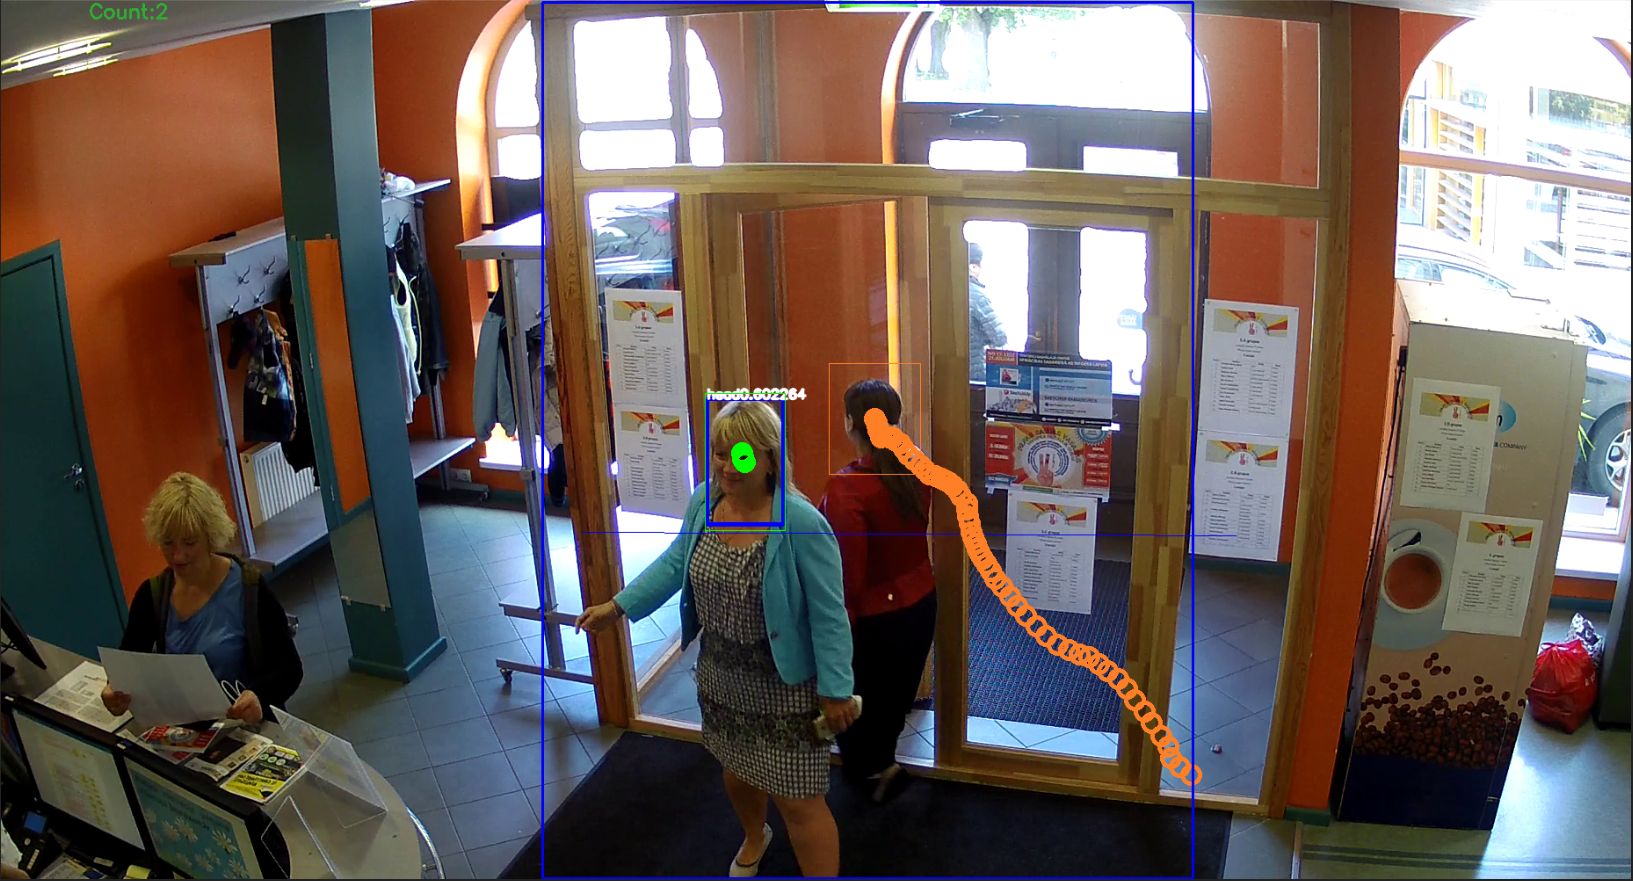
\includegraphics[height=6cm]{images/ssd1.png} %
	\caption{\textit{SSD} detektēšanas sistēma ar \textit{MIL} sekošanas algoritmu. Pirmais video.}%
	\label{fig:example}%
\end{figure}
\newpage
Attēlā 4.1. ar zilu krāsu atzīmēts sekošanas algoritmam interesējošais reģions. Ar oranžo krāsu atzīmētais ceļš norāda, ka sieviete attēla labajā pusē ir uztverta uzreiz kā sasniegts interesējošais reģions, taču ar zaļo krāsu atzīmētā sieviete ir uztverta vēlu. Vēlamais rezultāts ar zaļo krāsu atzīmēto sievieti uztvertu uzreiz kā tā parādītos durvīs, šajā gadījumā, detektēšana sievieti atradusi pāris kadrus vēlāk kā vēlams. Ir iespējams konfigurēt detektēšanas sistēmu, lai uztvertu objektus ar zemāku pārliecības slieksni, bet tas var izraisīt kļūdainus rezultātus, piemēram, atzīmēt cilvēku kāju kā galvu.

\begin{figure}[h]%
	\centering
	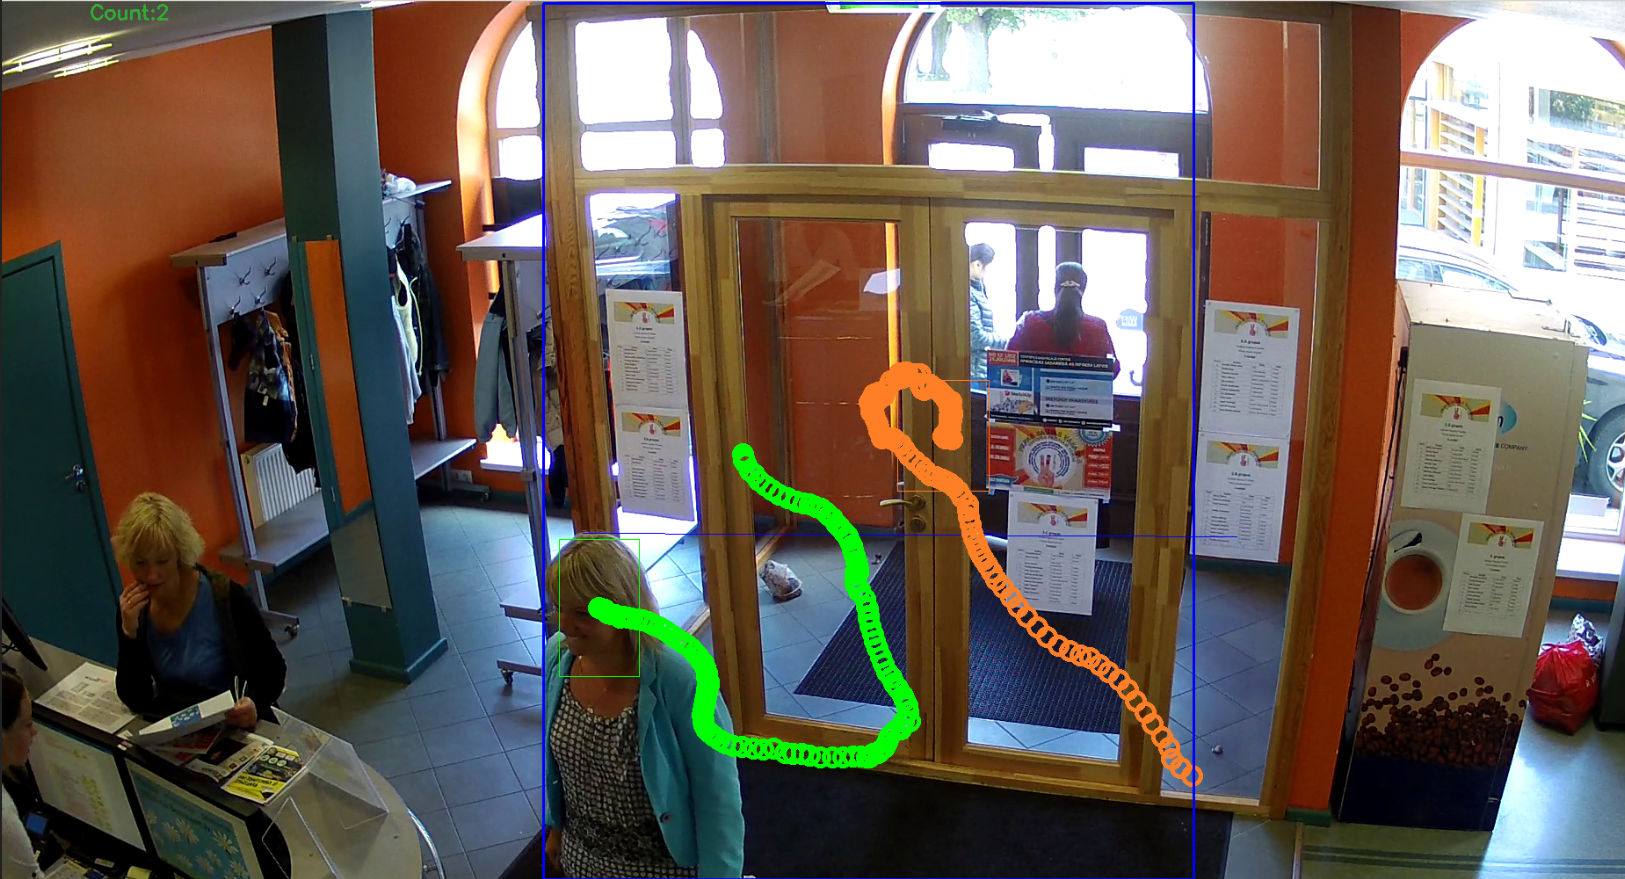
\includegraphics[height=6cm]{images/ssd2.png} %
	\caption{\textit{SSD} detektēšanas sistēma ar \textit{MIL} sekošanas algoritmu. Pirmais video.}%
	\label{fig:example}%
\end{figure}

Attēlā 4.2. attēlots brīdis pāris sekundes vēlāk, kad sieviete, kas attēlā 4.1. bija atzīmēta ar oranžo krāsu jau pametusi telpu, bet sekotājs apstājies pie durvīm. No tā var secināt, ka objektam pazūdot no sekošanas algoritma redzes loka, sekošanas algoritms pazaudē objektu un vairs nespēj to atrast. \textit{OpenCV} sekošanas programmējamā interfeisā piedāvātās metodes šādā brīdī nenorāda, ka objekts pazudis, bet uzskata, ka joprojām ir atrasts. Ar zaļo krāsu atzīmētajai sievietei, sekošanas algoritms ir veiksmīgi izsekojis līdz attēlā norādītajai atrašanās vietai, jo viņas ceļā nav bijuši šķēršļi. Vērts piebilst, ka dotais video fragments ir ļoti augstas izšķirtspējas, kas ļauj veikt objektu detektēšanu ar augstāku precizitāti. 

\begin{figure}[h]%
	\centering
	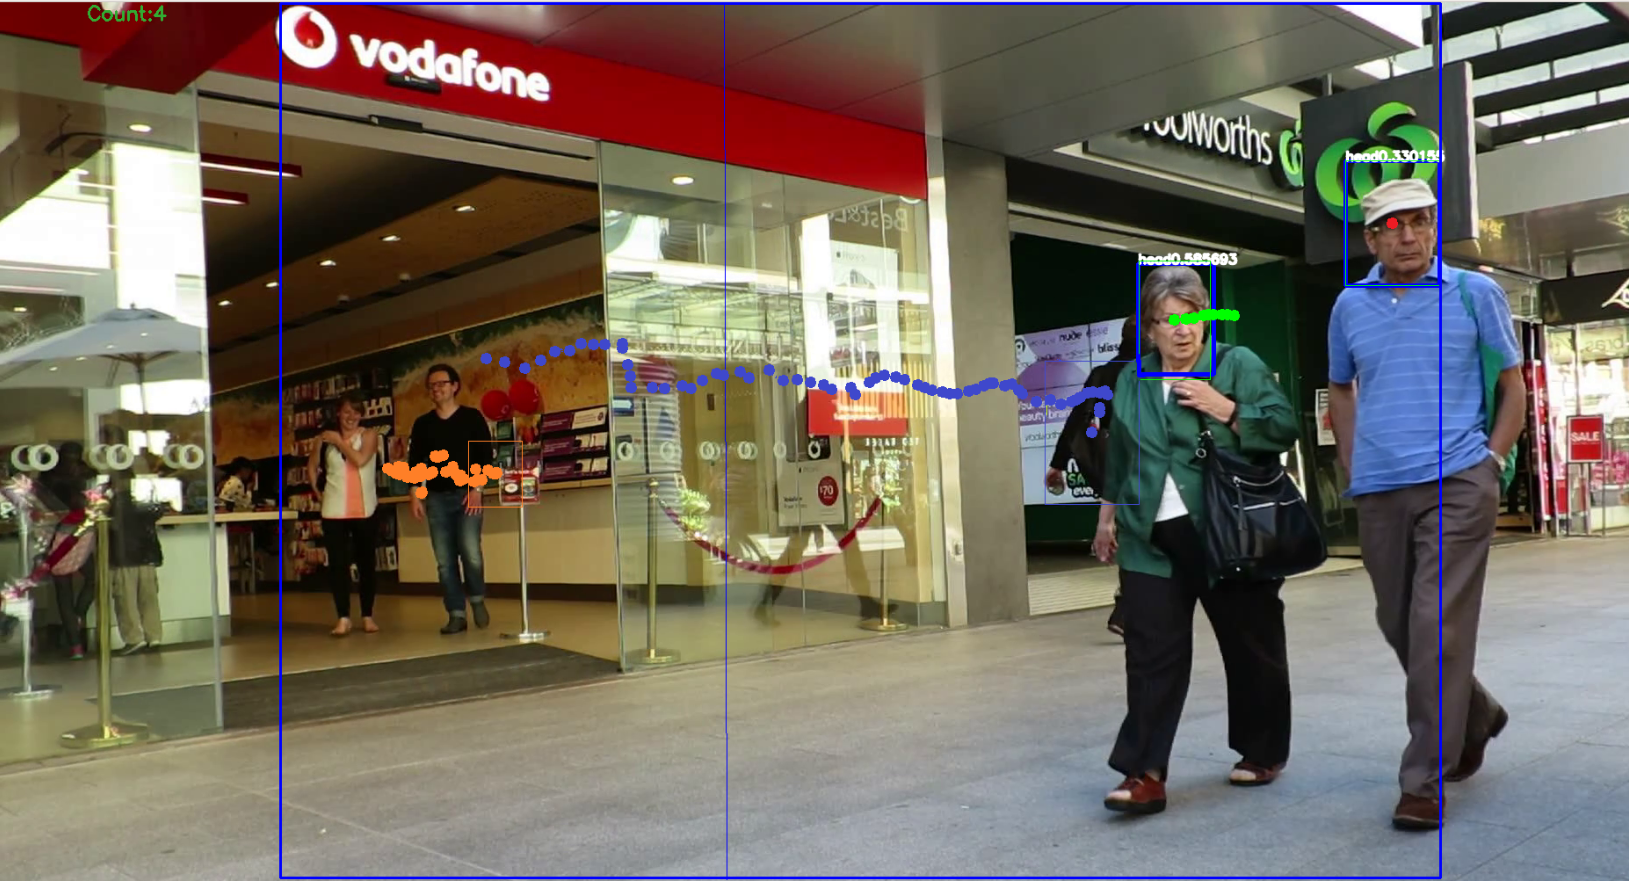
\includegraphics[height=6cm]{images/ssd3.png} %
	\caption{\textit{SSD} detektēšanas sistēma ar \textit{MIL} sekošanas algoritmu. Otrais video.}%
	\label{fig:example}%
\end{figure}

Attēlā 4.3. ir attēlots fragments no cita video, kas ir zemākas izšķirtspējas un filmēts citā vidē. Līdz dotajam brīdim, video fragmentā uztverti 4 objekti, kamēr 1 objekts no visiem nav atrasts. Ar oranžo,violeto un zaļo krāsu atzīmētie objekti ir uztverti pāris kadrus pēc tam, kad tie parādījušies interesējošajā reģionā, kamēr ar sarkano krāsu atzīmētais objekts uztverts uzreiz. Arī šajā gadījumā ir iespējams konfigurēt detektēšanas sistēmu, lai uztvertu objektus ar zemāku pārliecības slieksni, bet tas var izraisīt kļūdainus rezultātus, piemēram, atzīmēt cilvēku kāju kā galvu.

\begin{figure}[h]%
	\centering
	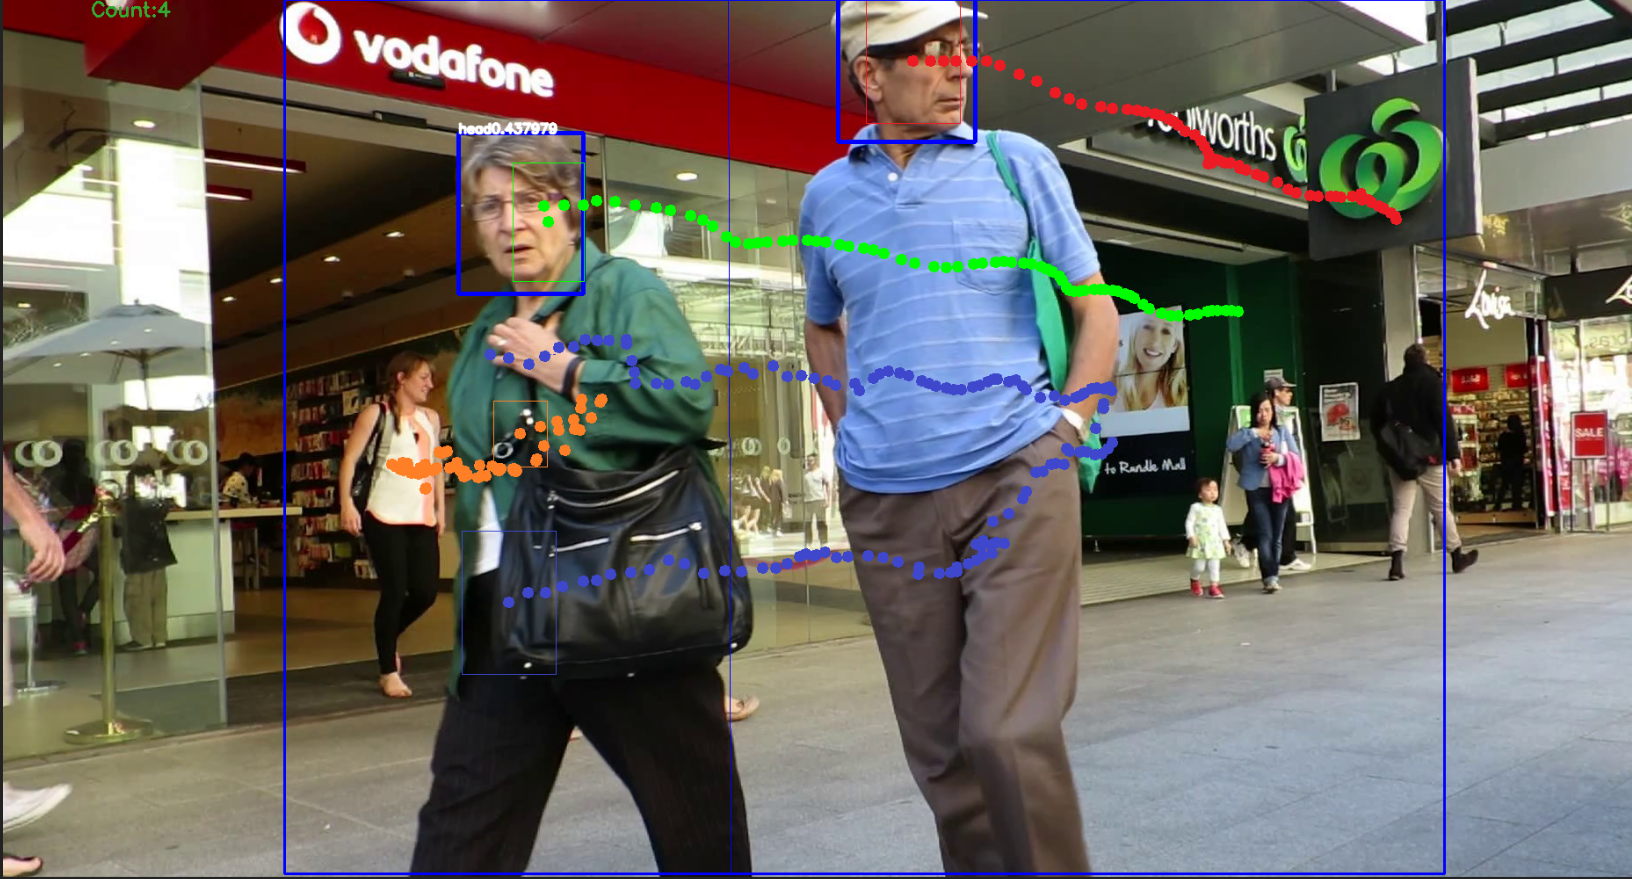
\includegraphics[height=6cm]{images/ssd4.png} %
	\caption{\textit{SSD} detektēšanas sistēma ar \textit{MIL} sekošanas algoritmu. Otrais video.}%
	\label{fig:example}%
\end{figure}

Līdz attēlā 4.4. redzamajam brīdim objektiem, kas ir tuvu filmēšanas punktam ir veiksmīgi izsekots, kamēr vīrietis, kas bija atzīmēts ar violeto krāsu vairs netiek uztverts un priekšplānā esošie objekti, šķērsojot to, lika sekošanas algoritmam kļūdīties un violetajam objektam atkal parādoties vairs nespēja tam izsekot. 

\begin{figure}[h]%
	\centering
	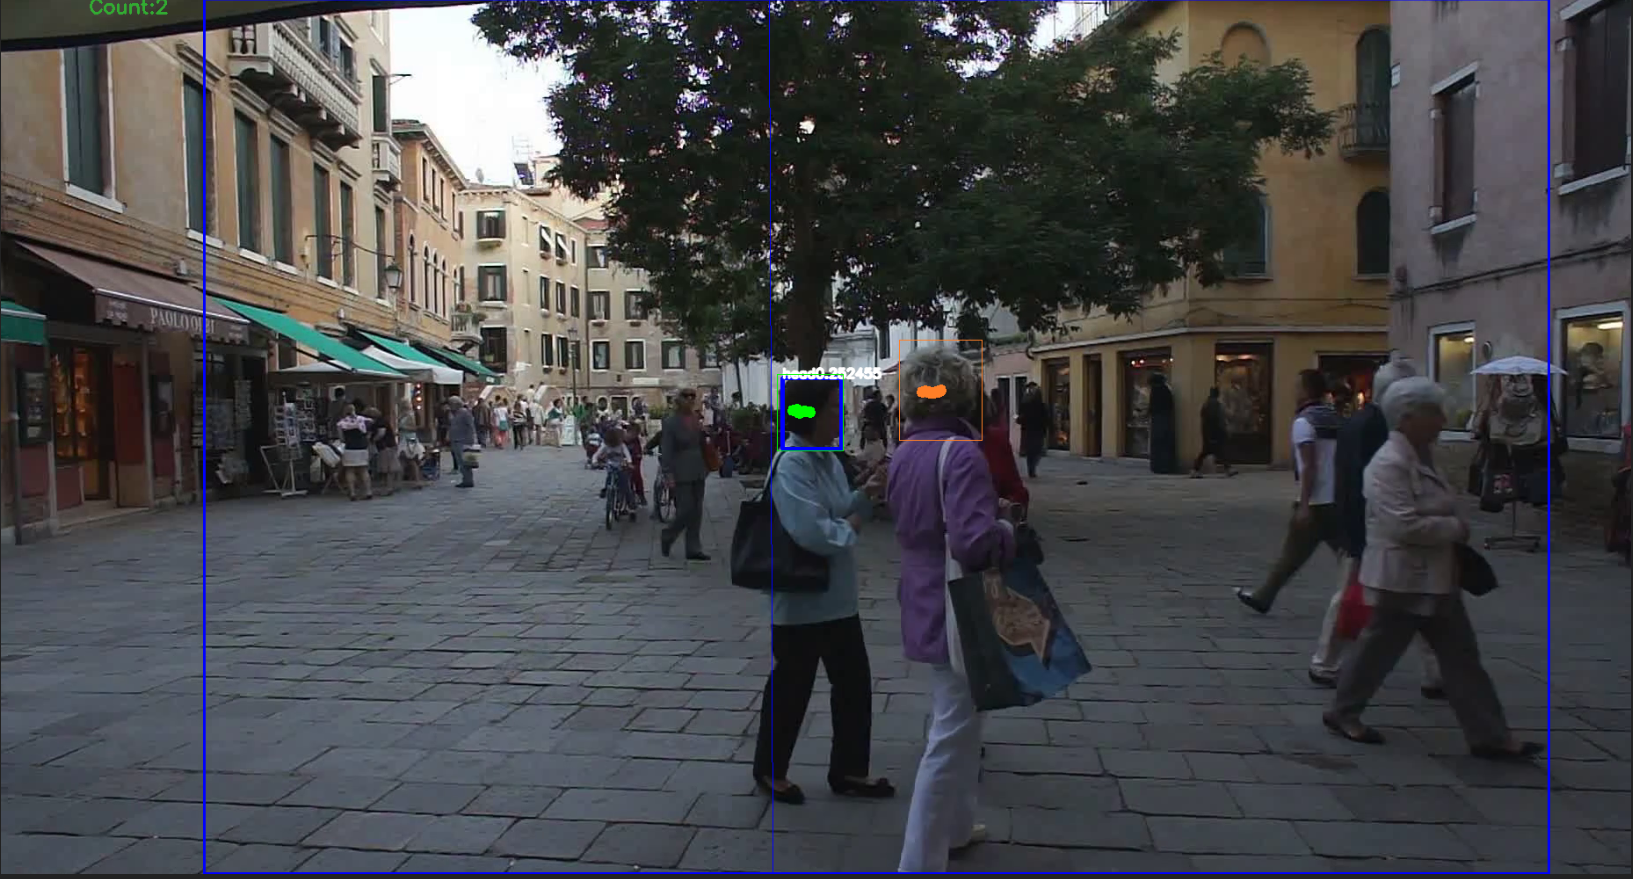
\includegraphics[height=6cm]{images/ssd5.png} %
	\caption{\textit{SSD} detektēšanas sistēma ar \textit{MIL} sekošanas algoritmu. Trešais video.}%
	\label{fig:example}%
\end{figure}

Attēlā 4.5. ir attēlots fragments no cita video, kas ir ļoti zemas izšķirtspējas un filmēts citā vidē. Dotais fragments ir pirmie video kadri, attēlā ir redzami daudz cilvēki, taču detektēšanas algoritms ir atradis tikai divus. Par iemeslu var uzskatīt ļoti zemo video fragmenta izšķirtspēju.

\begin{figure}[h]%
	\centering
	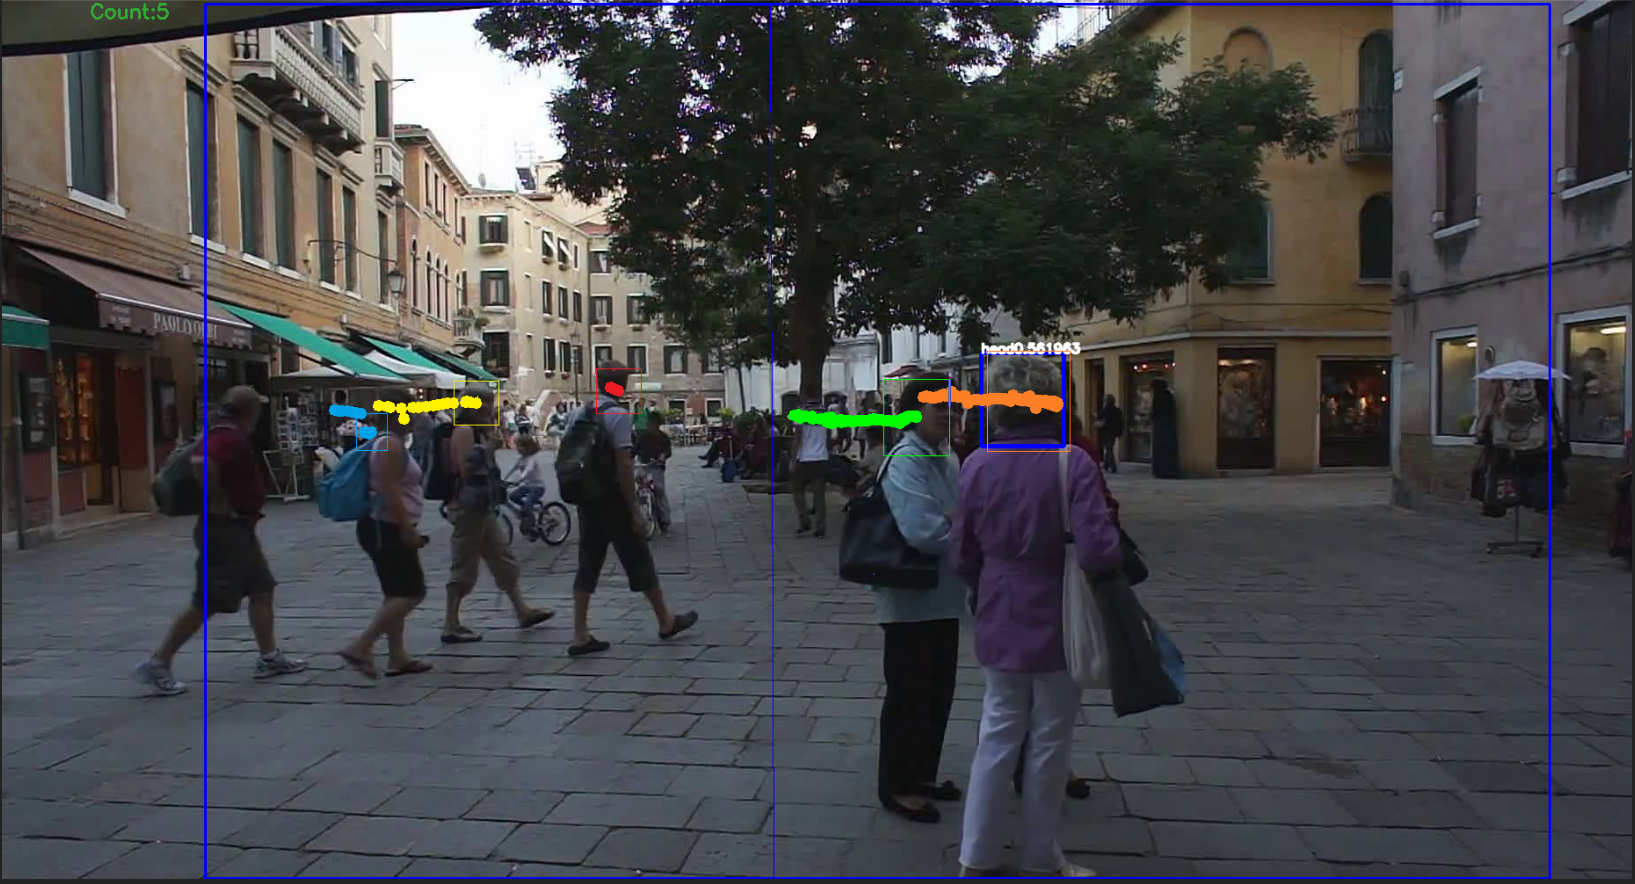
\includegraphics[height=6cm]{images/ssd6.png} %
	\caption{\textit{SSD} detektēšanas sistēma ar \textit{MIL} sekošanas algoritmu. Trešais video.}%
	\label{fig:example}%
\end{figure}

Attēlā 4.6. ir attēlots brīdis no tā paša video, pāris sekundes vēlāk, kad rāmī ir parādījušies un uztverti 3 jauni objekti. Detektēšana gan tiem nav notikusi līdz ar parādīšanos interesējošajā reģionā, bet pāris kadrus vēlāk. 

\textit{AdaBoost} sekošanas algoritms strādā gandrīz tik pat labi kā \textit{MIL} algoritms, brīžiem gan novērojami iztrūkumi, sekošanas laikā sekotājs brīžiem pazaudē objektu, bet ātri, pēc pāris kadriem, to atrod. Līdzīgi kā \textit{MIL} algoritmam, arī \textit{AdaBoost} netiek galā ar objektiem, kas video fragmentos novietojas aiz šķēršļiem, bet izpildes laikā ir ātrāks. Ja gala risinājumā nepieciešams izvēlēties starp \textit{MIL} un \textit{AdaBoost}, autors izvēlētos \textit{MIL}, jo, lai gan \textit{AdaBoost} ir nedaudz ātrāks, \textit{MIL} algoritms objektiem seko stabilāk.
\begin{figure}[h]%
	\centering
	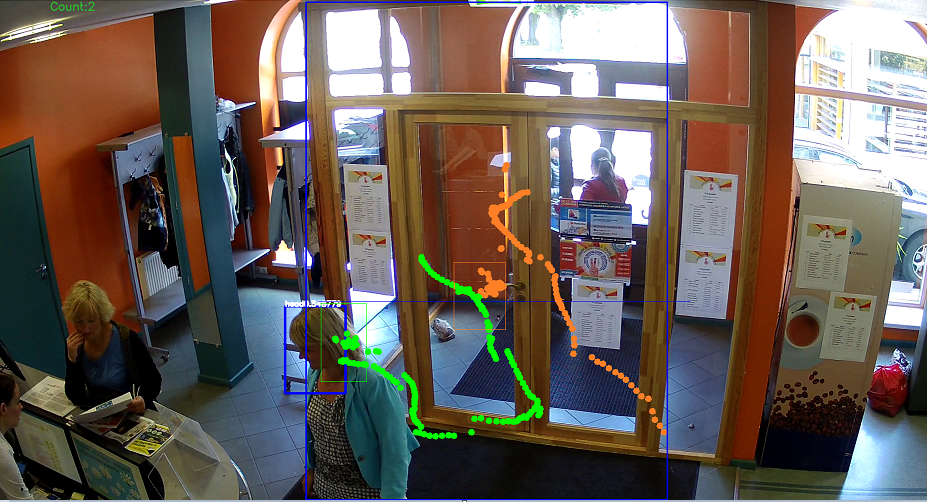
\includegraphics[height=6cm]{images/ssd7.png} %
	\caption{\textit{SSD} detektēšanas sistēma ar \textit{AdaBoost} sekošanas algoritmu. Pirmais video.}%
	\label{fig:example}%
\end{figure}
\paragraph{\textit{YOLO} detektēšanas sistēma ar \textit{OpenCV} sekošanas algoritmiem}
\hfill\par
Salīdzinot ar darba izstrādes laikā apmācīto \textit{SSD} objektu detektēšanas sistēmu, \textit{YOLO} detektēšanas sistēma tika apmācīta krietni mazāku laiku, kas arī atspoguļojās rezultātos. Augstas izšķirtspējas nekustīgos attēlos \textit{YOLO} detektēšanas sistēma rādīja labus rezultātus, taču video fragmentos detektēšanas kvalitāte bija zemāka kā \textit{SSD} detektēšanas sistēmai. Vēl viens iemesls salīdzinoši sliktākajai detektēšanas kvalitātei varētu būt praktiskā implementācija. Implementējot detektēšanu \textit{darknet} ietvarā, grūtības sagādāja no video fragmenta iegūto kadru pārveidošana uz \textit{darknet} \textit{Image} objektu. Tāda iemesla dēļ, pirms veikt detektēšanu, video fragmenti tika sadalīti attēlos un detektēšana tika veikta katram attēlam atsevišķi nevis \textit{OpenCV VideoFile} objektam kā \textit{SSD} gadījumā. Tādā veidā, sekošanas algoritms var pazaudēt savienojumus starp video kadriem.
\newpage
\begin{figure}[H]%
	\centering
	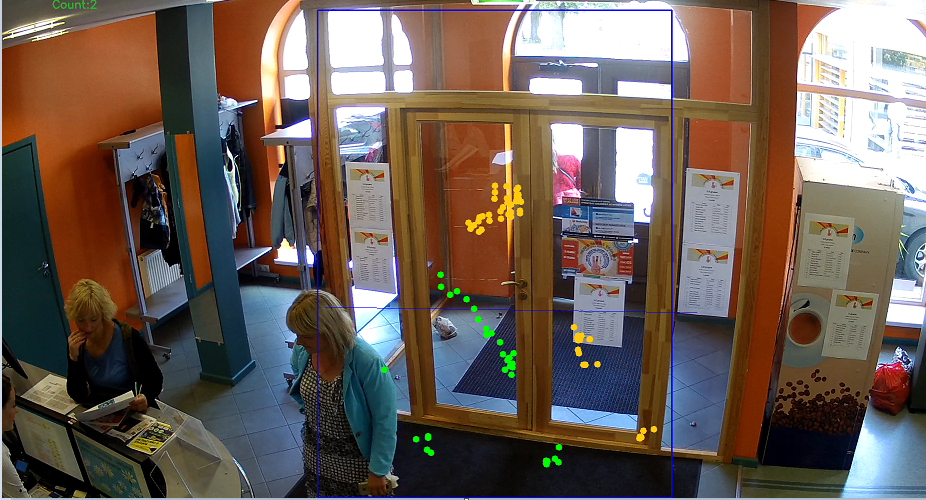
\includegraphics[height=5cm]{images/yolo1.png} %
	\caption{\textit{YOLO} detektēšanas sistēma ar \textit{AdaBoost} sekošanas algoritmu. Pirmais video.}%
	\label{fig:example}%
\end{figure}
\begin{figure}[H]%
	\centering
	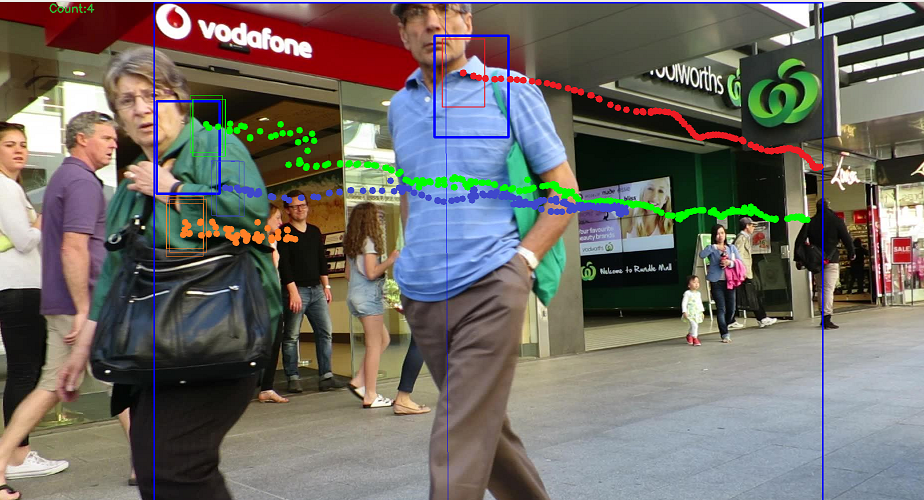
\includegraphics[height=5cm]{images/yolo2.png} %
	\caption{\textit{YOLO} detektēšanas sistēma ar \textit{AdaBoost} sekošanas algoritmu. Otrais video.}%
	\label{fig:example}%
\end{figure}
\begin{figure}[H]%
	\centering
	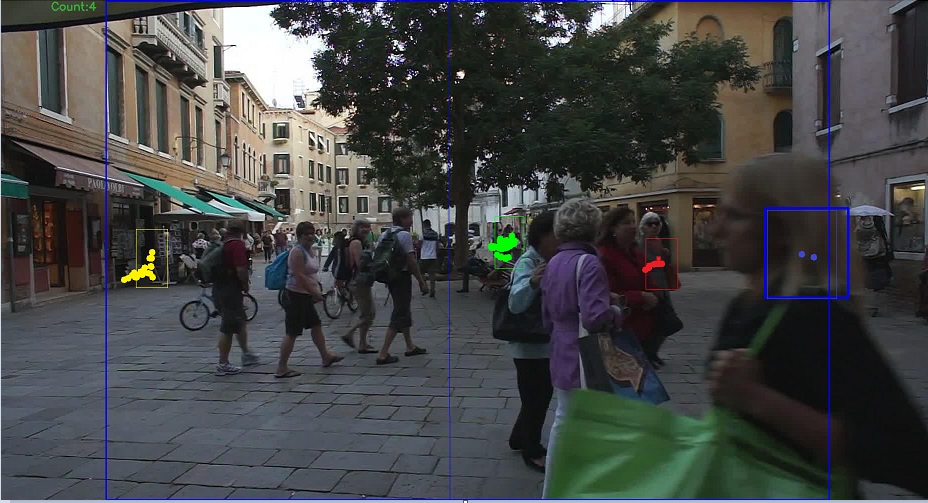
\includegraphics[height=5cm]{images/yolo3.png} %
	\caption{\textit{YOLO} detektēšanas sistēma ar \textit{AdaBoost} sekošanas algoritmu. Trešais video.}%
	\label{fig:example}%
\end{figure}
\newpage
Attēlā 4.8. var novērot, ka sekojot rodas iztrūkumi un detektēšana ir darbojusies līdzīgi \textit{SSD} detektēšanas sistēmai. Attēlā 4.9. priekšplānā esošie cilvēki ir detektēti labāk kā \textit{SSD} sistēmai, taču fonā esošie netiek atrasti. Kā jau darbā minēts, \textit{YOLO} slikti detektē mazus objektus, kas varētu būt iemesls. Sekošanas algoritms attēlā 4.9. darbojas līdzīgi kā \textit{MIL} sekošanas algoritms, kur objekti, aizklājot citus, pārtvēra to ierobežojošos logus. 

Tā kā video fragments attēlā 4.10. ir ļoti zemas izšķirtspējas, visi objekti ir salīdzinoši mazi, kas \textit{YOLO} sagādā lielas problēmas. Fona esošais objekts ir atrasts veiksmīgi, bet pārējie cilvēki, kas pārvietojas fonā tiek detektēti ļoti vāji.
\chapter{Secinājumi un priekšlikumi}
\paragraph{Secinājumi}
\hfill\par
\begin{enumerate}
	\item 
	\item 
	\item 
	\item 
	\item 
	\item 
	\item 
	\item 
	\item 
	\item 
	\item 
	\item 
	\item 
	\item 
	\item 
	\item 
	\item 
	\item 
	\item 
	\item 
	\item 
	\item 
	\item 
	\item 
	\item 
\end{enumerate}
\paragraph{Priekšlikumi}
\hfill\par
\begin{enumerate}
	\item 
	\item 
	\item 
	\item 
	\item 
	\item 
	\item 
	\item 
	\item 
	\item 
	\item 
	\item 
	\item 
	\item 
	\item 
	\item 
	\item 
	\item 
	\item 
	\item 
	\item 
	\item 
	\item 
	\item 
	\item 
\end{enumerate}